\documentclass[UTF8]{ctexart}
\title{2021年盘锦市数学中考部分题图}
\author{M81}
\date{\today}
\usepackage{tikz}
\usepackage{tkz-euclide}
\begin{document}
\maketitle
\begin{figure}[htbp]
    \centering
    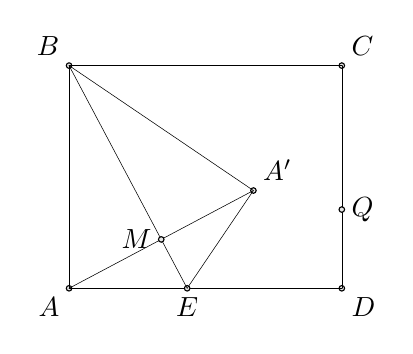
\begin{tikzpicture}
    \tkzDefPoints{0/0/A,0/2*{sqrt(2)}/B,2*{sqrt(3)}/2*{sqrt(2)}/C,2*{sqrt(3)}/0/D}
    \tkzDrawPoints(A,B,C,D)
    \tkzLabelPoint[below left](A){$A$}
    \tkzLabelPoint[above left](B){$B$}
    \tkzLabelPoint[above right](C){$C$}
    \tkzLabelPoint[below right](D){$D$}
    \tkzDrawSegments(A,B B,C C,D D,A)
    \tkzDefPoints{1.5/0/E,2*{sqrt(3)}/1/Q}
    \tkzDrawPoints(E,Q)
    \tkzLabelPoint[below](E){$E$}
    \tkzLabelPoint[right](Q){$Q$}
    \tkzDrawSegment(B,E)
    \tkzDefPointBy[reflection=over B--E](A) \tkzGetPoint{A'}
    \tkzDrawPoint(A')
    \tkzLabelPoint[above right](A'){$A'$}
    \tkzDrawSegments(A',B A',E A,A')
    \tkzInterLL(A,A')(E,B) \tkzGetPoint{M}
    \tkzDrawPoint(M)
    \tkzLabelPoint[left](M){$M$}
    \end{tikzpicture}
    \caption{填空最后一道题}
    \label{fig:my_label}
\end{figure}

\begin{figure}[htbp]
    \centering
    \begin{tikzpicture}
    \tkzDefPoints{0/0/A,2/0/O,4/0/B,2/2/F,1/0/D}
    \tkzDrawPoints(A,B,O,F,D)
    \tkzLabelPoint[left](A){$A$}
    \tkzLabelPoint[below](O){$O$}
    \tkzLabelPoint[right](B){$B$}
    \tkzLabelPoint[above left](F){$F$}
    \tkzLabelPoint[above left](D){$D$}
    \tkzDrawCircle(O,A)
    \tkzDefPointOnCircle[angle=307,center=O,radius=2 cm] \tkzGetPoint{C}
    \tkzDrawPoint(C)
    \tkzLabelPoint[below right](C){$C$}
    \tkzDrawSegments(A,B B,C A,C B,O F,C)
    \tkzInterLL(A,C)(D,F) \tkzGetPoint{G}
    \tkzDrawPoint(G)
    \tkzLabelPoint[below left](G){$G$}
    \tkzDefLine[perpendicular=through B](A,B) \tkzGetPoint{Z}
    \tkzInterLL(D,F)(B,Z) \tkzGetPoint{E}
    \tkzDrawPoint(E)
    \tkzLabelPoint[right](E){$E$}
    \tkzDrawSegments(E,B G,E)
    \end{tikzpicture}
    \caption{圆}
    \label{fig:my_label}
\end{figure}

\begin{figure}[htbp]
    \centering
    \begin{tikzpicture}
    \tkzDefPoints{0/0/A,3/0/B,3/3/C,0/3/D}
    \tkzDefPointOnCircle[angle=165,center=B,radius=1.6 cm] \tkzGetPoint{E}
    \tkzDefLine[perpendicular=through B](E,B) \tkzGetPoint{Z}
    \tkzInterLC(Z,B)(B,E) \tkzGetPoint{F}
    \tkzDefMidPoint(E,F) \tkzGetPoint{G}
    \tkzDefLine[parallel=through D](E,F) \tkzGetPoint{Y}
    \tkzDefLine[parallel=through F](D,G) \tkzGetPoint{X}
    \tkzInterLL(D,Y)(F,X) \tkzGetPoint{H}
    \tkzDrawPoints(A,B,C,D,E,F,G,H)
    \tkzDrawSegments(A,B B,C C,D D,A B,E B,F E,F D,G H,F D,H H,C C,G)
    \tkzLabelPoints[left](A,D,E)
    \tkzLabelPoints[right](B,C,F)
    \tkzLabelPoint[above](H){$H$}
    \tkzLabelPoint[left](G){$G$}
    \end{tikzpicture}
    \caption{倒数第二道大题}
    \label{fig:my_label}
\end{figure}

\begin{figure}[htbp]
    \centering
    \begin{tikzpicture}
    \tkzInit[xmin=-2.7,xmax=4.7,ymin=-3,ymax=5]
    \tkzDrawXY[noticks]
    \draw[domain=-2.2:4.2] plot(\x,{-0.5*(\x)^2+\x+4});
    \draw[domain=-0.5:4] plot(\x,{\x-2});
    \tkzDefPoints{0/0/O,-2/0/A,4/0/B,0/4/C,0/-2/D,2/0/E,2.4/3.52/P}
    \tkzInterLL(D,E)(B,C) \tkzGetPoint{F}
    \tkzInterLL(B,O)(P,F) \tkzGetPoint{Q}
    \tkzDefLine[perpendicular=through P](C,B) \tkzGetPoint{Z}
    \tkzInterLL(P,Z)(B,C) \tkzGetPoint{M}
    \tkzDefLine[perpendicular=through Q](C,B) \tkzGetPoint{Y}
    \tkzInterLL(Q,Y)(B,C) \tkzGetPoint{N}
    \tkzDrawLine(B,C)
    \tkzDrawPoints(A,B,C,D,E,F,P,Q,M,N)
    \tkzDrawSegments(P,Q P,M Q,N)
    \tkzLabelPoints[above right](P,N,B)
    \tkzLabelPoints[below](E,Q,M)
    \tkzLabelPoints[left](C,F)
    \tkzLabelPoint[above left](A){$A$}
    \tkzLabelPoint[below left](O){$O$}
    \tkzLabelPoint[right](D){$D$}
    \end{tikzpicture}
    \caption{最后一道大题}
    \label{fig:my_label}
\end{figure}

\end{document}